% author:   sam tenka
% create:   2022-02
% change:   2022-02

%==============================================================================
%=====  0.  DOCUMENT SETTINGS  ================================================
%==============================================================================

%~~~~~~~~~~~~~~~~~~~~~~~~~~~~~~~~~~~~~~~~~~~~~~~~~~~~~~~~~~~~~~~~~~~~~~~~~~~~~~
%~~~~~~~~~~~~~  0.0. About and Beyond this Exposition  ~~~~~~~~~~~~~~~~~~~~~~~~

%---------------------  0.0.0. page geometry  ---------------------------------
\documentclass[12pt]{article}
\usepackage[top=3cm, bottom=3cm, left=3.5cm, right=2.5cm]{geometry}

%---------------------  0.0.1. math packages  ---------------------------------
\usepackage{amsmath, amssymb, amsthm, mathtools, bm, moresize, euler}
%\usepackage[lite]{mtpro2}
 
%---------------------  0.0.2. graphics packages  -----------------------------
\usepackage{graphicx, epsdice, xcolor, float, wrapfig, caption}

%~~~~~~~~~~~~~~~~~~~~~~~~~~~~~~~~~~~~~~~~~~~~~~~~~~~~~~~~~~~~~~~~~~~~~~~~~~~~~~
%~~~~~~~~~~~~~  0.1. Header Formatting  ~~~~~~~~~~~~~~~~~~~~~~~~~~~~~~~~~~~~~~~

%---------------------  0.1.0. section header style  --------------------------

\definecolor{mblu}{rgb}{0.05, 0.40, 0.70}
\definecolor{mblulite}{rgb}{0.60, 0.80, 0.90}
\newcommand{\msec}[1]{\subsection*{\color{mblu}\textsf{#1}}}
\newcommand{\mpar}[1]{%
    %\indent\par\raisebox{0cm}[0cm][0cm]{\makebox[0cm]{\hspace{-4.75cm}\parbox{2.5cm}{\raggedleft\color{mblu}\textsf{#1}}}}%
    \makebox[0cm]{\hspace{-4.75cm}\parbox{2.5cm}{\raggedleft\color{mblulite}\textsf{#1}}}%
}

%---------------------  0.1.1. clear the bibliography's header  ---------------
\usepackage{etoolbox}
\patchcmd{\thebibliography}{\section*{\refname}}{}{}{}

%~~~~~~~~~~~~~~~~~~~~~~~~~~~~~~~~~~~~~~~~~~~~~~~~~~~~~~~~~~~~~~~~~~~~~~~~~~~~~~
%~~~~~~~~~~~~~  0.2. Math Symbols and Blocks  ~~~~~~~~~~~~~~~~~~~~~~~~~~~~~~~~~

%---------------------  0.2.0. caligraphic letters  ---------------------------
\newcommand{\Dd}{\mathcal{D}}
% ...
\newcommand{\Hh}{\mathcal{H}}
% ...
\newcommand{\Ll}{\mathcal{L}}
\newcommand{\Mm}{\mathcal{M}}
\newcommand{\Nn}{\mathcal{N}}
\newcommand{\Oo}{\mathcal{O}}
\newcommand{\Pp}{\mathcal{P}}
% ...
\newcommand{\Ss}{\mathcal{S}}
% ...
\newcommand{\Xx}{\mathcal{X}}

%---------------------  0.2.1. double struck letters  -------------------------
\newcommand{\CC}{\mathbb{Z}}
% ...
\newcommand{\NN}{\mathbb{N}}
% ...
\newcommand{\PP}{\mathbb{P}}
\newcommand{\QQ}{\mathbb{Q}}
\newcommand{\RR}{\mathbb{R}}
% ...
\newcommand{\ZZ}{\mathbb{Z}}

%---------------------  0.2.2. math environments  -----------------------------
\newtheorem*{qst}{Question}
\newtheorem*{thm}{Theorem}
\newtheorem*{lem}{Lemma}
% ...
\theoremstyle{definition}
\newtheorem*{dfn}{Definition}

%---------------------  0.2.3. math objects  ----------------------------------
\newcommand{\enc}{\text{enc}}
\newcommand{\dec}{\text{dec}}

%~~~~~~~~~~~~~~~~~~~~~~~~~~~~~~~~~~~~~~~~~~~~~~~~~~~~~~~~~~~~~~~~~~~~~~~~~~~~~~
%~~~~~~~~~~~~~  0.3. Title  ~~~~~~~~~~~~~~~~~~~~~~~~~~~~~~~~~~~~~~~~~~~~~~~~~~~

\begin{document}

{
    \centering \Huge \sf \color{mblu} 
    Coding Theory in a Nutshell
    \vspace{0.5cm}
}

%==============================================================================
%=====  1.  INTRO  ============================================================
%==============================================================================

The 20th century was the century of higher dimensions.  Positions became phase
spaces; species, ecosystems; voltages, signals.  With large dimensions came new
geometry --- curvature, catastrophes, concentration --- geometry underpinning
the technologies of that age.  We'll tell the story of how concentration of
measure led to dense ball packing and thus to astonishingly efficient
communication.

Following Shannon, we'll formalize protocols for redundantly communicating long
signals across noisy channels.  We seek concise (small redundancy), reliable
(small error rate) protocols.  As entropy clearly lower bounds concision, we
ask: how does reliability deteriorate as we approach that bound?  For example,
how loose is the concision bound among very-reliable protocols?  That bound
eludes all low-dimensional examples we'll make by hand.  And yet the bound is
tight: miraculously, there are protocols arbitrarily close to the entropic
bound with arbitrarily low error-rate!

Shannon's 1948 miracle is strikingly non-constructive: it gives no concrete
optimal protocol.  It would take another 2 billion seconds of dogged hunt for
workers to construct a provably optimal protocol.  After sketching this hunt's
history, we'll construct that protocol, analogize to fast fourier transforms,
and handwaive optimality.

\msec{A Noisy Channel}

    \indent\par
    \mpar{redundancy}%
    Say we have a channel across which we transmit a stream of $0$s and $1$s.
    Alas, each transmitted bit has an independent chance $p=1-q<1/2$ of
    flipping to the other value.  Thus, to communicate some length-$N$ message
    $m\in 2^N$, we transmit some longer, \emph{coded} bitstring
    $y=\enc(m)\in 2^{RN}$.  Here $R\in [1,\infty)$ is the
    \emph{redundancy}.  The receiver decodes a corrupted bitstring $\hat y = y
    \oplus z$, which it decodes via $\hat m = \dec(\hat y) \in 2^N$.
    This pair $(\enc, \dec)$ is our \emph{communication protocol},
    or \emph{code}. 
    $$
         m  \xrightarrow{\enc}
         y  \xrightarrow{\oplus z}
    \hat y  \xrightarrow{\dec}
    \hat m
    $$

    \mpar{error rate}%
    We seek concise (low $R$), reliable (low $\epsilon$) protocols.
    Here $\epsilon$ is the chance of decoding $m$ incorrectly
    averaged uniformly over all messages:
    $$
        \epsilon =
        \PP_m \PP_z \left[m = \dec(\enc(m)\oplus z) \right] 
    $$
    We minimize $\epsilon$ with respect to a given encoder by decoding each
    received $\hat y$ to a minimum $\dec(\hat y) = \arg \min
    \delta(\enc(\hat m), \hat y)$ of the hamming distance.  We'll by
    default assume this $\dec$; algorithmic concerns may
    suggest other decoders.

    \mpar{distance}%
    We say our code enjoys \emph{minimum distance} and \emph{radius}:
    $$
        \delta_\star = \min_{m \neq m^\prime} \delta(\enc(m), \enc(m^\prime))
        \quad
        \quad
        \quad
        r_\star = \lceil\delta_\star/2\rceil
    $$
    With $S^n_p = \sum_{0\leq k<n} {RN \choose k} p^k q^{RN-k}$ the chance of
    less than $k$ corruptions, we bound
    $$
        p^{r_\star} q^{NR-r_\star} / 2^N
        \leq
        \epsilon \leq 1-S^{r_\star}_p
    $$
    For any fixed code, this \emph{binomial bound} tightens as $p\to 0$:
    $\epsilon \in \Theta(p^{r_\star})$.  

\msec{Protocols Matter}

    \indent\par
    \mpar{linear}%
    A rich class of protocols arise with $\enc$ an injective
    linear map $:2^{N}\to 2^{RN}$; here, we regard the domain and codomain as
    vector spaces over the field with $2$ elements.  Due to linearity (and
    injectivity), the minimum distance coincides with the minimum hamming
    norm $|y|$ among images of nonzero messages.

    A representative case is $N=32$, $RN=9\cdot 32$, $p=1/20$.  That is, we
    wish to communicate four bytes --- perhaps a word in a novel --- by
    transmitting thirty six bytes, knowing that roughly fourteen bits
    will get corrupted.  How small can we get $\epsilon$?

    \mpar{repetition}%
    What first comes to mind is the \emph{repetition code}
    $$
        y=\enc(m)=(m,m,m, m,m,m, m,m,m)
    $$
    We decode each bit of $m$ by taking the majority value among the $9$
    received estimates of that bit.
    %
    We get a bit wrong only when at least $5$ estimates are corrupted (relatedly,
    $\delta_\star=5$).  The
    estimates are mutually independent and each estimate has error rate linear
    in $p$ as $p\to 0$, so $\epsilon \sim 32{9\choose 5} p^5 \sim 1.3\cdot
    10^{-3}$.  We expect our novel to have an error every couple pages.

    \mpar{pairwise}%
    But we can use our redundancy more effectively!  Let
    $$
        y=\enc(m)=(m,Wm)
    $$
    where $W$, a $(16\cdot 16)\times 32$ matrix, gives for each ``even-odd''
    pair $(2i,2j+1) \in [0,16)^2$ the sum $m_{2i}\oplus m_{2j+1}$.  Intuitively, $W$
    ``mixes up'' $m$'s bits, diluting each corruption across $m$'s many bits
    until it is correctible.

    One way to decode the bit $\hat m_0$ from $\hat y = (\tilde m,
    \tilde{Wm})$ is to take the majority value among the $17$ estimates
    $$
        \tilde m_0
        \quad
        \quad
        \tilde m_1\oplus (\widetilde{Wm})_{(0,1)}
        \quad
        \quad
        \tilde m_3\oplus (\widetilde{Wm})_{(0,3)}
        \quad
        \quad
        \cdots
    $$
    Likewise to decode the other bits.
    %
    We get a bit wrong only when at least $9$ estimates are corrupted
    (relatedly, $\delta_\star=9$).  The estimates are mutually independent and
    each estimate has error rate linear in $p$ as $p\to 0$, so $\epsilon \sim
    32\left(2^4{8\choose 4} + 2^5{8\choose 5}\right) p^9 \sim 4 \cdot 10^{-5}$, a
    drastic improvement over the repetition code.  We expect only a few errors
    in our novel.

    % TODO: figure of log(error rate) vs log(p) for both codes 

\msec{A Beautiful Code}

    \indent\par
    \mpar{hamming}
    Imagine a simplex on $k$ vertices.  There are ${k \choose d+1}$ cells
    of dimension $d$.  Take $0\leq D<k$; call cells of dimension $d<D$
    \emph{parity cells} and the remaining cells \emph{data cells}.
    For each labeling of data cells by bits, we get a labeling of parity cells
    by bits: we label each p-cell by the mod-2 sum of the labels of the
    containing d-cells.
    %
    % TODO: consider modification so that turned-on dim2 p-cells affect dim1
    %       p-cells???   More elegant analysis...??? ( see below )
    %
    We regard the full labeling as a bitstring of
    length $2^k-1$.  Let $N$ count the data cells, let $RN = 2^k-1$ count all
    cells, and let $\enc$ send a data labeling to a full labeling.  This
    gives us a \emph{generalized Hamming code}.

    For example, with $D=1$, we get the classic Hamming codes with
    $(N,RN,\delta_\star) = (2^k-1-k,2^k-1,3)$.  That $\delta_\star\geq 3$
    reflects that if every atom appears in an even number of members of a
    nonempty set $\Ss$ of sets, then $\Ss$ has size at least $3$.  We may thus
    correct any single corruption.

    Higher $D$s give codes robust to more corruptions.
    For example, $(k,D)=(5,2)$ gives a $(16,31,6)$ code??????
    %
    That $\delta_\star\geq 5$ reflects that if every size-$\leq 2$ set includes
    into an even number of members of a nonempty set $\Ss$ of sets, then $\Ss$
    has size at least $5$.
    %
    Indeed, $\Ss$ must have size at least $3$ by above. 

%==============================================================================
%=====  2.  BOUNDS  ===========================================================
%==============================================================================

\msec{Obstructions to Concise, Reliable Codes}

% GRAPH:
% https://www.desmos.com/calculator/kxpggoe8xo
% https://www.desmos.com/calculator/wphanl7oyd
% https://www.desmos.com/calculator/das4d1l9pp
% https://www.desmos.com/calculator/lmoddgzogm
% https://www.desmos.com/calculator/com1zvnbwl

    \indent\par
    \mpar{entropy}%
    Which tuples $N, RN, p, \epsilon$ are feasible?  Let $\Delta$ denote the
    vector difference $\Delta=m-\hat m$.  
    Then $(\hat y, \Delta)$ determines
    $
        (m,z) = (\dec(\hat y)\oplus\Delta, \hat y - \enc(m))
    $.
    So, by subadditivity, data processing, and independence:
    $$
        H(\hat y)+H(\Delta)
        \geq
        H(\hat y,\Delta)
        \geq
        H(m,z)
        =
        H(m)+H(z) 
    $$
    Plugging in $H(\hat y)\leq RN$,
    %$H(\Delta) \leq H(\epsilon) + \epsilon N$,
    $H(\Delta) \leq H(\epsilon)N$,
    $H(m)=N$, and
    $H(z)=H(p)RN$, we see
    $$
        R \geq \frac{1-H(\epsilon)}{1-H(p)}
    $$
    In particular, we need $R \geq 1/(1-H(p))$ to have any hope
    of a small $\epsilon$.

    %$N(1-H(\epsilon))$ informative bits.  But
    %after corruption, our transmission carries only $RN(1-H(p))$ informative
    %bits.  
    %%
    %So:
    %$$
    %    R\geq \frac{1-H(\epsilon)}{1-H(p)}
    %$$
    %%
    
    \mpar{volume}%
    Besides the entropy bound, there are ball packing obstructions.  Indeed, to
    get good rates for small $p$, we want large $r_\star$s.  We want to pack
    $2^N$ --- but by additivity of volume can pack at most $1/S^r_{1/2}$ ---
    disjoint (open) hamming-balls of radius $r$. 

    In more detail: the median ball's volume is at most $2^{NR}\cdot 2^{N-1}$. 
    In turn,
    the volume is at least ${NR\choose r}$ for any specific closed $r$-ball.
    So at least half of the balls have closed radii obeying
    $
        2^{NR}/2^{N-1} \geq {NR\choose r}
    $
    or, by a Stirling approximation,
    $$
        1-(N-1)/NR \geq H(r/(NR)) 
    $$
    For this median $r$ we have
    $
        \epsilon \geq (1/2) p^{r+1}q^{NR-r-1} 
    $.

    \mpar{geometry}%
    Perhaps most interestingly, the hypercube's metric structure prevents us
    from achieving the volume bound.
    %
    First, when $2^N \geq 3$ we must have $\delta_\star \leq (2/3) RN$.
    This is due to the hypercube's positive curvature; for,
    $\delta(a,z),\delta(b,z)\geq (1/2 + x)RN$ implies $\delta(a,b)\leq
    (1-2x)RN$.
    Though the volume bound allows $N,RN,\delta_\star=2,7,5$, this curvature
    bound does not.

    We may extend this idea to slightly smaller $x=\delta_\star/(RN)$.  How
    many length-$RN$ bitstrings have distance at least $xRN$ from the
    $RN$-zeros string and from the $(1-x)RN$-ones-then-$xRN$-zeros string?
    The exact count is:
    \begin{align*}
        \sum_{0\leq sRN\leq (1-x)RN} % number of zeros to turn into ones
        \sum_{0\leq tRN\leq    x RN} % number of ones to turn into zeros 
        [\![s\geq t]\!]              % don't decrease total number of ones
        [\![s+t\geq x]\!]            % change enough bits
        {(1-x)RN \choose sRN}
        {xRN \choose tRN}
    \end{align*}
    The summand is maximized near $s=x/2=t$ at which point
    it has log roughly:
    $$
        N \leq \left(H\left(\frac{1}{2}\frac{x}{1-x}\right)(1-x) + x\right) RN
    $$
    Say $y=x/(1-x)=1/(1/x-1)$, $x=1/(1+1/y)=y/(1+y)$, $1-x=1/(1+y)$.
    Then $1/R \leq (H(y/2)+y)/(1+y) \leq 2/3 + (2-y)^{3/4}/2$,
    so $2-(2(1/R-2/3))^{4/3} \geq y$, whence we get an upper bound on $x$.
    
    \mpar{a map}%

    %\begin{figure}[H]
    %    \centering
    %    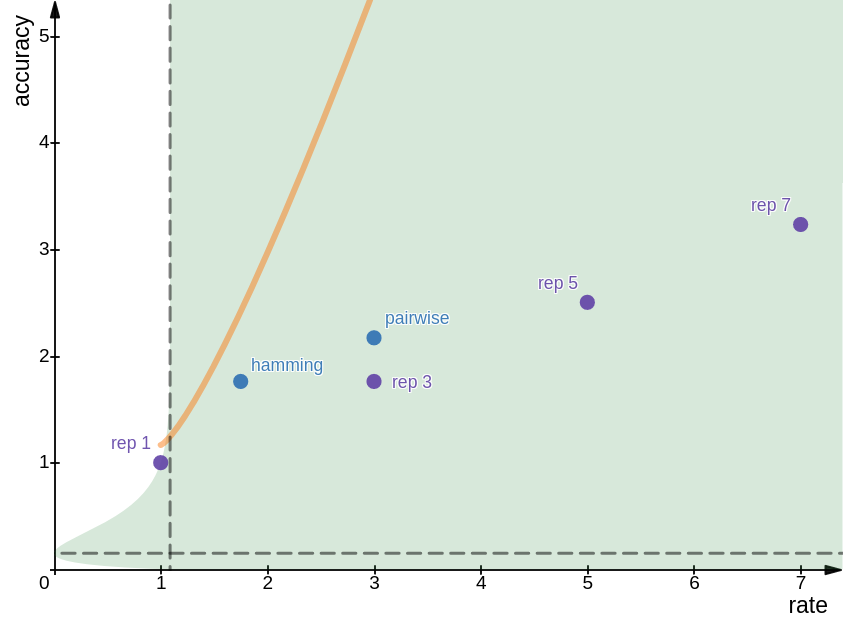
\includegraphics[width=13.0cm]{coding-map-N8-p0.01-vert100}
    %    \caption{{
    %        Feasible accuracy-rate pairs for $N=8, p=10^{-2}$.
    %        Here, accuracy is $\alpha=\log_p(\epsilon)/N$; it is as if for each
    %        message bit we flip a $p$-weighted coin $\alpha$ times and we
    %        successfully communicate that bit unless they all come up heads.
    %        Thus, the identity code (``repeat once'') has accuracy and
    %        rate both equal to one.
    %        %
    %        In purple are the repetition codes; in blue, the hamming code and
    %        the pairwise code we encountered earlier.
    %        %
    %        Shaded in green are the pairs allowed by the entropy bound.
    %        Pairs above the orange curve are forbidden by the volume bound.
    %    }}
    %\end{figure}


    %Let's plot normalized accuracy $\alpha = (1-\epsilon)^{1/N}$ (vertically)
    %vs normalized redundancy $\rho = R(1-H(p))-1$ (horizontally).  We chose our
    %normalizations to unite a code $m\mapsto \enc(m)$ with its double
    %$(m,n)\mapsto(\enc(m),\enc(n))$.

    %The entropic bound says
    %$\alpha \leq 2^{\rho}$, which is vacuous for $1\leq \rho$.  Note that $\rho$
    %can be as low as $-1$, where we have coin flip chances $\alpha=1/2$. 

    %Meanwhile, we have
    %$(qp)^{r_\star} \leq \epsilon$
    %and ${RN \choose r_\star} \leq 2^{RN-N}$.
    %Assuming Stirling is an equality and assuming $r\ll RN$ and being cavalier:
    %and $RN\lg(RN) - r\lg r - (RN-r)lg(RN-r) \leq RN-N$ 
    %and $r\lg(RN/r) \leq RN-N$ 
    %and $r \leq (R-1)N/\lg(R/(R-1))$ 
    %and $r \leq SN/\lg(1+1/S)$ 
    %Here $S=R-1$.
    %%
    %Take the interesting regime $S\approx 0$ so $\lg(1+1/S) \approx -\lg(S)$.
    %Assume very small $p$ and hence very small $H(p)$ so $S\approx \rho$.
    %Note $(qp)^r$ is decreasing in $r$. 
    %$$
    %    \epsilon^{1/N} \geq p^{-Slg(S)} \approx p^{-\rho \lg(\rho)} 
    %$$

    %$$
    %    \epsilon^{1/N} \geq p^{-Slg(S)} \approx p^{-\rho \lg(\rho)} 
    %$$

    %$$
    %    \alpha \leq 1 - \epsilon/N 
    %           \leq 1 - (p^{-\rho \lg(\rho)})^N/N 
    %$$

\msec{A Miracle}

%==============================================================================
%=====  3.  POLAR CODES  ======================================================
%==============================================================================

\msec{Polar Codes}
\msec{Analysis of Polar Codes}

\msec{Appendix A: Entropy and Binomials}
    Here, $H(z) = z\lg(\frac{1}{z}) +
    (1-z)\lg(\frac{1}{1-z})$ is \emph{entropy}. 

    Stirling says that ${T \choose xT} \sim 2^{H(x)T} / \sqrt{2\pi x(1-x)T}$,
    or, for small $x$:
    $$
        \lg{{T \choose xT}} \approx H(x)T - \frac{1}{2} \lg(xT) - 0.66 
    $$
    This is good plus-minus $0.50$ for $1\leq xT\leq T/4$.

    We find it useful to bound binomial sums.  For $x < 1/2$:
    FIXX
    \begin{align*}
        &
        q^{xT} \sum_{0\leq i\leq xT} {T\choose i} (p/q)^{i}
        \\ \leq &
        \left(\frac{qx}{(1-x)}\right)^{xT} \cdot
        \sum_{0\leq i\leq xT} {T\choose xT} \left(\frac{(1-x)p}{xq}\right)^i 
        \\ \leq &
        \left(\frac{qx}{(1-x)}\right)^{xT} \cdot
        {T \choose xT} \cdot \frac{xq}{xq-(1-x)p} 
    \end{align*}

%\msec{Appendix A: Shannon 1948}
%\msec{Appendix B: Gallager 1960}
%\msec{Appendix C: Arikan 2008}

\end{document}



%\msec{Bonus: A Beautiful Code}%: 4-7-3 Hamming}
%
%    \indent\par
%    \mpar{visualization}%
%    We can can visualize points in small-dimensional
%    hypercubes $2^{NR}$ as combinatorial structures on the standard cube $2^3$.  
%    For instance, each $2$-tuple (think: arrow) of $2^3$'s points represents a
%    vertex of $2^6$.  If we insist that the first entry is a point on a fixed
%    square face, we get $2^5$.  If instead we mark each arrow as dashed or
%    solid, we get $2^7$.  
%
%    \mpar{hamming}%
%    Say $N=4$, $NR=7$.  $R$ is too small for even a full repetition.  Can we
%    nevertheless correct any singleton
%    corruption $|z|=1$?  That is, can we get $\delta_\star\geq 3$?
%    %
%    Yes!   
%    %
%    We want sixteen points on a $7$-D hypercube with every two points separated
%    by a distance of at least $3$.
%    %
%    Let's use the kernel of $P:2^7\to 2^3$ given by
%    %$P(C,B,a,A,b,c,z) =
%    $P(a,b,c,A,B,C,z) =
%    (a+b+C+z, a+B+c+z, A+b+c+z)$.  Figure 1 (left) shows this code's
%    symmetry.
%    
%    \mpar{reduced}%
%    We may pass from $(N,NR,\delta_\star)=(4,7,3)$
%                  to $(3,6,3)$
%    by setting $z=0$ in the hamming code.
%    Note that this reduced code outperforms the comparable repeat-twice code's
%    $(3,6,2)$; reduced hamming, unlike repetition, can
%    always correct a single corruption ($|z|=1$)!
%    %
%    Reduced hamming puts eight points on a $6$-D cube with every two points
%    separated by a distance of at least $3$.  We get it if we take just the
%    green arrows in Figure 1 (left).  It helps to visualize the tetrahedron
%    with vertices at the green loops.
%
%    Figure 1 (center) gives another $(3,6,3)$ code.  In what sense is it
%    the same as reduced hamming?
%
%    \begin{figure}[H]
%        \centering
%        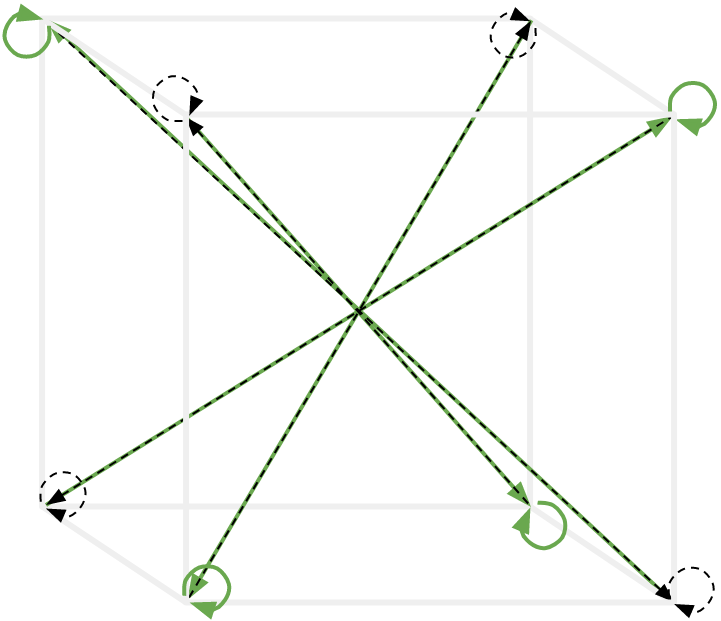
\includegraphics[height=4.0cm]{4-7-3-code}
%        \quad
%        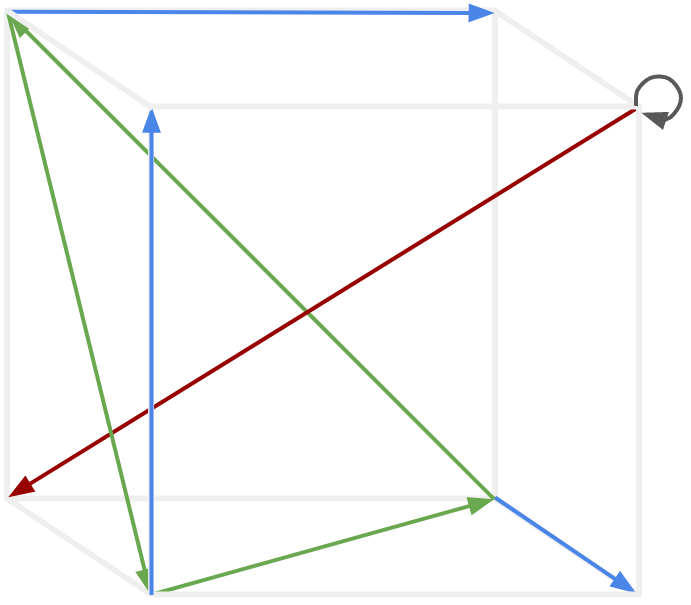
\includegraphics[height=4.0cm]{3-6-3-code}
%        %\quad
%        %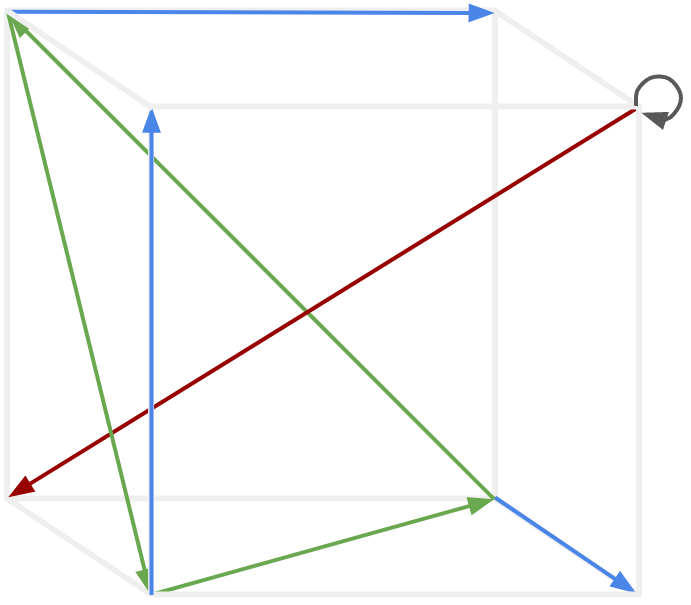
\includegraphics[height=4.0cm]{3-6-3-code}
%        \caption{{
%            Our $(4,7,3)$ code.
%            Our $(3,6,3)$ code.
%            %Our $(2,9,5)$ code.
%        }}
%    \end{figure}
%
%
%
%%==============================================================================
%%=====  2.  BOUNDS  ===========================================================
%%==============================================================================
%
%\msec{Obstructions to Concise, Reliable Codes}
%
%% GRAPH:
%% https://www.desmos.com/calculator/kxpggoe8xo
%% https://www.desmos.com/calculator/wphanl7oyd
%
%    \indent\par
%    \mpar{entropy}%
%    Which tuples $N, RN, p, \epsilon$ are feasible?  To achieve error
%    $\epsilon$ we must communicate $N(1-H(\epsilon))$ informative bits.  But
%    after corruption, our transmission carries only $RN(1-H(p))$ informative
%    bits.  Here, $H(z) = z\lg(\frac{1}{z}) +
%    (1-z)\lg(\frac{1}{1-z})$ is \emph{entropy}. 
%    %
%    So:
%    $$
%        R\geq \frac{1-H(\epsilon)}{1-H(p)}
%    $$
%    %
%    In particular, we need $R \geq 1/(1-H(p))$ to have any hope of a small
%    $\epsilon$.
%    
%    \mpar{volume}%
%    Besides the entropy bound, there are geometric obstructions.  Indeed, to
%    get good rates for small $p$, we want large $r_\star$s.  We want to pack
%    $2^N$ --- but by additivity of volume can pack at most $2^N\leq
%    1/S^r_{1/2}$ --- disjoint (open) hamming-balls of radius $r$. 
%    % TODO: rates!!
%
%    In more detail: the median ball's volume is at most $2^{NR}/N$.  In turn,
%    the volume is at least ${NR\choose r}$ for any specific closed $r$-ball.
%    So at least half of the balls have closed radii obeying
%    $
%        2^{NR}/2^N \geq {NR\choose r}
%    $
%    or, by a Stirling approximation,
%    $$
%        1-1/R \geq H(r/(NR)) 
%    $$
%    For this median $r$ we have
%    $
%        \epsilon \geq (1/2) p^{r+1} 
%    $.
%
%    \mpar{shape}%
%    Perhaps most interestingly, the balls' \emph{shape} prevents us from 
%    achieving the volume bound.  Take $2^N=3$, $2^{NR}=16$, for instance.
%    %
%    Can we get $\delta_\star\geq 3$?  The volume bound allows this.
%    %
%    And yet we cannot pack eight open $2$-balls into the hypercube $2^4$.
%    %
%    For if two points are antipodes, then the third will be too close to one
%    of the two; and if no points are antipodes, then all pairs have distance
%    $3$, which is impossible since the hypercube is bipartite.
%
%    Or, take $N=2$, $NR=7$.  
%    %
%    Can we get $\delta_\star\geq 5$?  The volume bound allows this.
%    %
%    And yet we cannot pack four open $3$-balls into the hypercube $2^7$. 
%    For, without loss one of the points is all zeros and every other point has
%    at least $5$ ones.  But two of the latter points will share at least $3$ of
%    those ones and hence be too close to each other.
%    %
%    Intuitively, this comes from the hypercube having small diameter.
%
%    As a last example, let $N=3$, $NR=9$. 
%    %
%    Can we get $\delta_\star\geq 5$?  The volume bound allows this.
%    %
%    And yet we cannot pack eight open $3$-balls into the hypercube $2^9$. 
%    %
%    For, without loss one of the points is all zeros and every other point has
%    at least $5$ ones.  Say point $x$ is $a\geq 5$ ones followed by $9-a$ ones. 
%    And say point $x$ is...
%
%    %000000000
%    %000111111
%    %111000111
%    %111111000
%
%    ......
%    ......
%    ......
%    ......
%    ......
%    ......
%    ......
%    ......
%    ......
%    ......
%
%    %TODO: figure.
%
%    \mpar{a map}%
%
%    \begin{figure}[H]
%        \centering
%        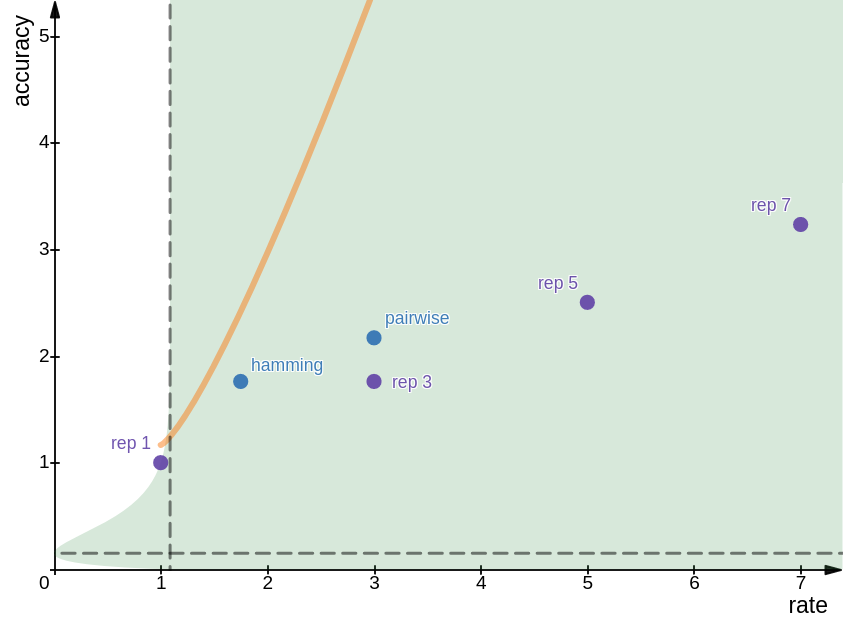
\includegraphics[width=13.0cm]{coding-map-N8-p0.01-vert100}
%        \caption{{
%            Feasible accuracy-rate pairs for $N=8, p=10^{-2}$.
%            Here, accuracy is $\alpha=\log_p(\epsilon)/N$; it is as if for each
%            message bit we flip a $p$-weighted coin $\alpha$ times and we
%            successfully communicate that bit unless they all come up heads.
%            Thus, the identity code (``repeat once'') has accuracy and
%            rate both equal to one.
%            %
%            In purple are the repetition codes; in blue, the hamming code and
%            the pairwise code we encountered earlier.
%            %
%            Shaded in green are the pairs allowed by the entropy bound.
%            Pairs above the orange curve are forbidden by the volume bound.
%        }}
%    \end{figure}
%
%
%    %Let's plot normalized accuracy $\alpha = (1-\epsilon)^{1/N}$ (vertically)
%    %vs normalized redundancy $\rho = R(1-H(p))-1$ (horizontally).  We chose our
%    %normalizations to unite a code $m\mapsto \enc(m)$ with its double
%    %$(m,n)\mapsto(\enc(m),\enc(n))$.
%
%    %The entropic bound says
%    %$\alpha \leq 2^{\rho}$, which is vacuous for $1\leq \rho$.  Note that $\rho$
%    %can be as low as $-1$, where we have coin flip chances $\alpha=1/2$. 
%
%    %Meanwhile, we have
%    %$(qp)^{r_\star} \leq \epsilon$
%    %and ${RN \choose r_\star} \leq 2^{RN-N}$.
%    %Assuming Stirling is an equality and assuming $r\ll RN$ and being cavalier:
%    %and $RN\lg(RN) - r\lg r - (RN-r)lg(RN-r) \leq RN-N$ 
%    %and $r\lg(RN/r) \leq RN-N$ 
%    %and $r \leq (R-1)N/\lg(R/(R-1))$ 
%    %and $r \leq SN/\lg(1+1/S)$ 
%    %Here $S=R-1$.
%    %%
%    %Take the interesting regime $S\approx 0$ so $\lg(1+1/S) \approx -\lg(S)$.
%    %Assume very small $p$ and hence very small $H(p)$ so $S\approx \rho$.
%    %Note $(qp)^r$ is decreasing in $r$. 
%    %$$
%    %    \epsilon^{1/N} \geq p^{-Slg(S)} \approx p^{-\rho \lg(\rho)} 
%    %$$
%
%    %$$
%    %    \epsilon^{1/N} \geq p^{-Slg(S)} \approx p^{-\rho \lg(\rho)} 
%    %$$
%
%    %$$
%    %    \alpha \leq 1 - \epsilon/N 
%    %           \leq 1 - (p^{-\rho \lg(\rho)})^N/N 
%    %$$
%
%


%Say we pack $1+k$ points into $2^{RN}$ at distances all at least $d_\star$.
%    Without loss, one point is all zeros; then each other point has at least
%    $d_\star$ of its bits equal to one.  
%
%    We thus
%    have at least $kd_\star$ ones total.  But at most $NR$ of those ones are
%    turned on in only one point; each of the remaining $kd_\star-NR$ ones is
%    turned on in at least two points.  Thus, some two points must share at
%    least $(kd_\star-NR)/{k \choose 2}$ ones.  But by hypothesis, they share
%    at most $NR-d_\star$ ones.  In short, with $x=d_\star/(RN) \in (0,1]$:
%    $$
%        \frac{kx-1}{{k \choose 2}} \leq 1-x
%        \quad
%        %(\frac{2}{k-1}+1)x \leq \frac{2}{k(k-1)}+1
%        %\quad
%        %k(2+k-1)x \leq 2+k^2-k
%        \quad
%        x \leq \frac{k^2-k+2}{k^2+k}
%        %\quad
%        %k=2: x \leq 4/6
%        %k=3: x \leq 8/12
%        %k=4: x \leq 14/20
%    $$
%
%
%%Take $2^N=3$, $2^{RN}=16$, for instance.
%%    %
%%    Can we get $\delta_\star\geq 3$?  The volume bound allows this.
%%    %
%%    And yet we cannot pack eight open $2$-balls into the hypercube $2^4$.
%%    %
%%    For if two points are antipodes, then the third will be too close to one
%%    of the two; and if no points are antipodes, then all pairs have distance
%%    $3$, which is impossible since the hypercube is bipartite.
%%
%%    Or, take $N=2$, $NR=7$.  
%%    %
%%    Can we get $\delta_\star\geq 5$?  The volume bound allows this.
%%    %
%%    And yet we cannot pack four open $3$-balls into the hypercube $2^7$. 
%%    For, without loss one of the points is all zeros and every other point has
%%    at least $5$ ones.  But two of the latter points will share at least $3$ of
%%    those ones and hence be too close to each other.
%%    %
%%    Intuitively, this comes from the hypercube having small diameter.


